\begin{frame} {Definition of a manipulation planning problem}
  \parbox{.39\linewidth} {
    \begin{itemize}
    \item grippers (frames attached to a joint),
    \item handles (frames attached to a joint),
    \item contact surfaces
    \end{itemize}
    define grasps and stable poses for objects.
  }
  \parbox{.59\linewidth} {
    \begin{center}
      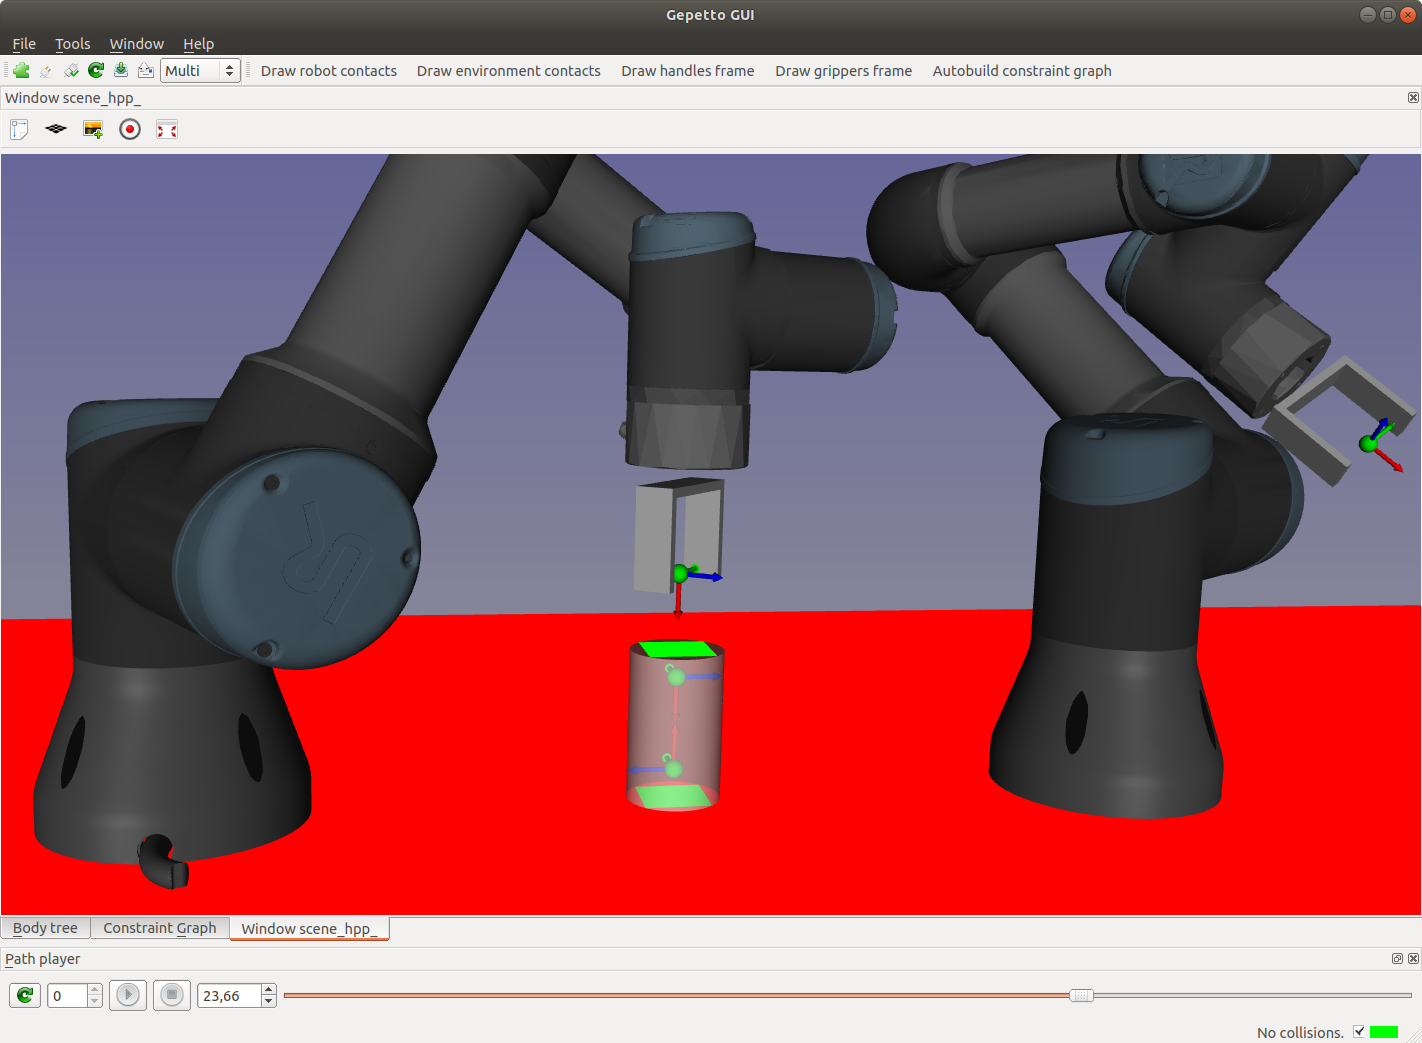
\includegraphics[width=\linewidth]{figures/manipulation-problem.png}
    \end{center}
  }
\end{frame}

\begin{frame} {The factory}
  \parbox{.39\linewidth} {
  Given all the possible grasps (defined by grippers and handles), a factory builds the constraint
  graph with all possible states
  }
  \parbox{.59\linewidth} {
    \begin{center}
      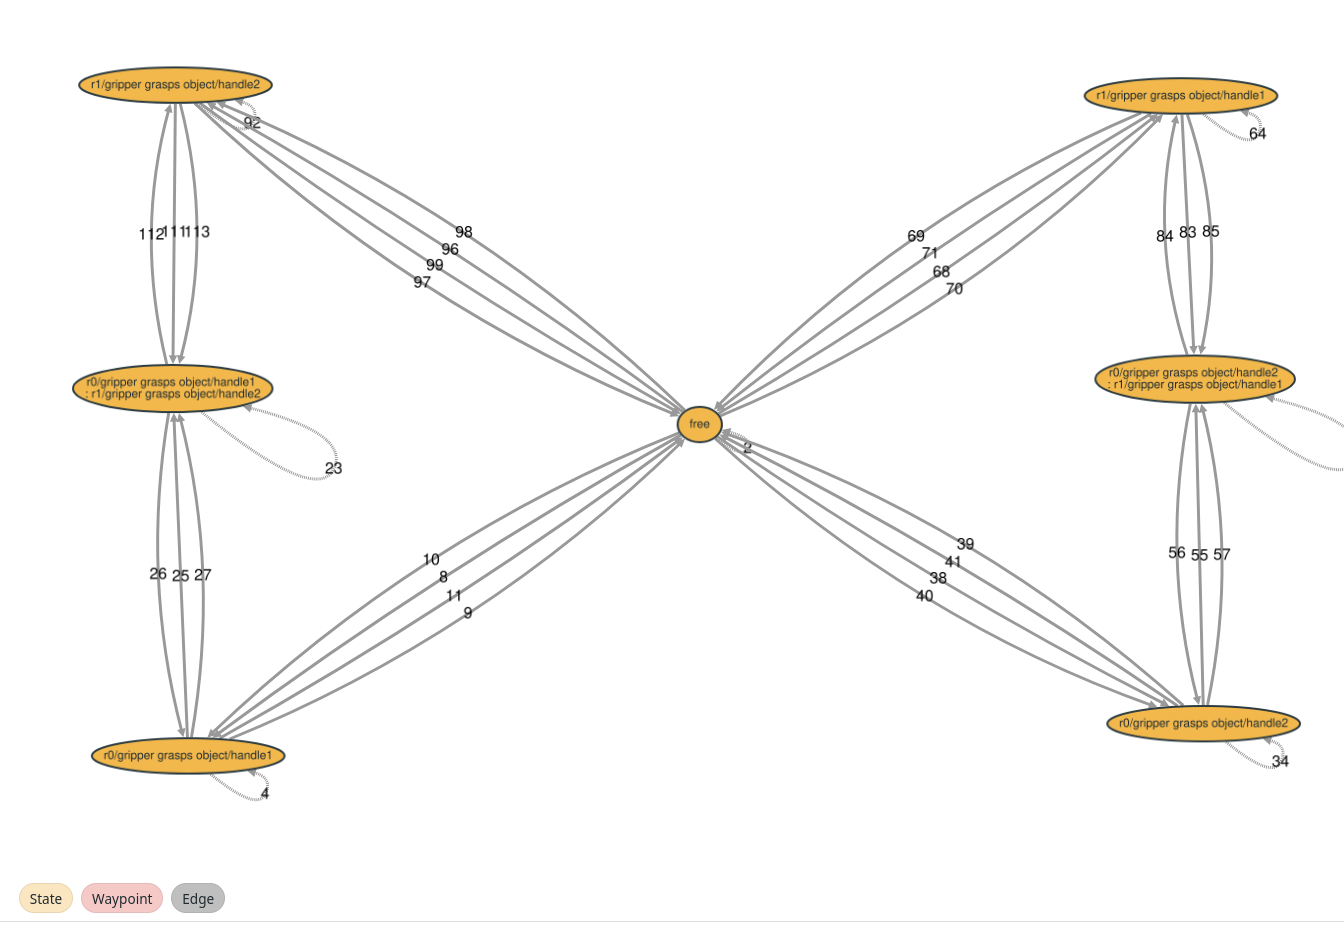
\includegraphics[width=\linewidth]{figures/constraint-graph-raw.png}
    \end{center}
  }
\end{frame}

\begin{frame} {Waypoint transitions and states}
  \parbox{.59\linewidth} {
    To ease manipulation planning resolution, some intermediate states are inserted by the factory.
  }
  \parbox{.39\linewidth} {
    \begin{center}
      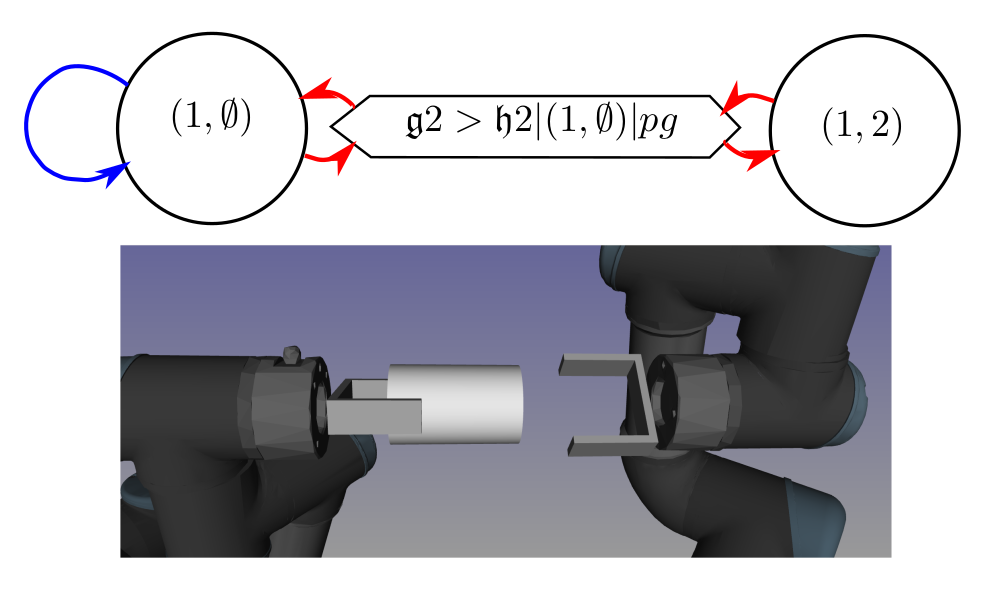
\includegraphics[width=\linewidth]{figures/waypoint-1.png}
      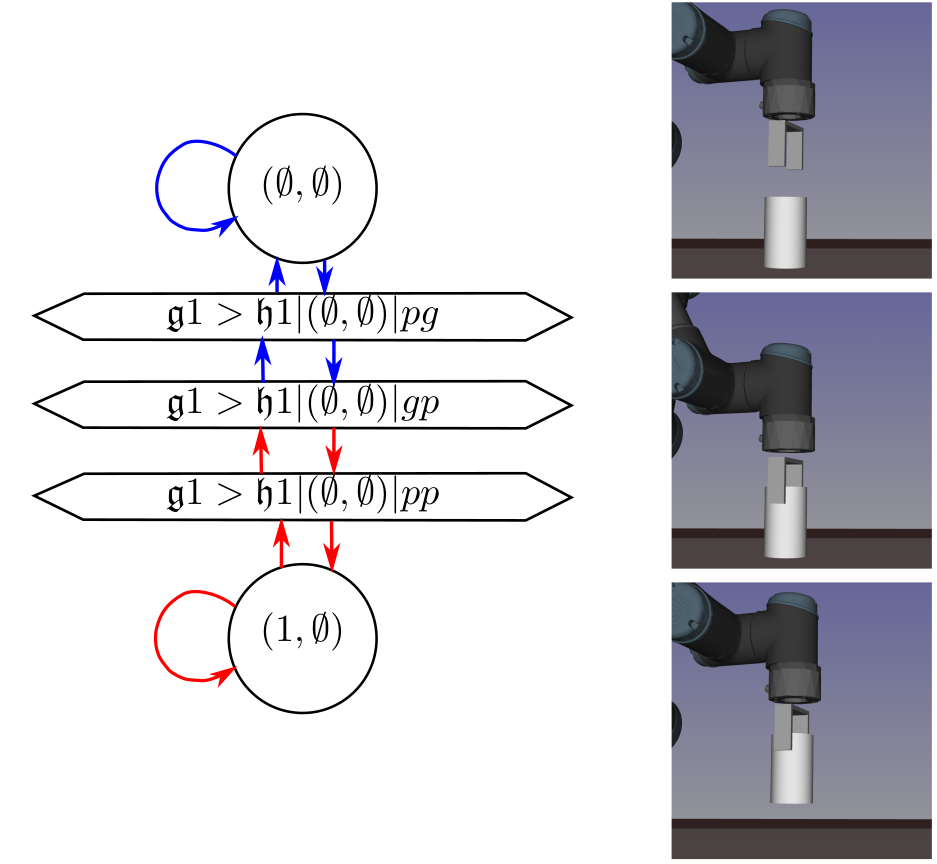
\includegraphics[width=\linewidth]{figures/waypoints-3.png}
    \end{center}
  }
\end{frame}

\begin{frame} {Waypoint transitions and states}
  \begin{center}
    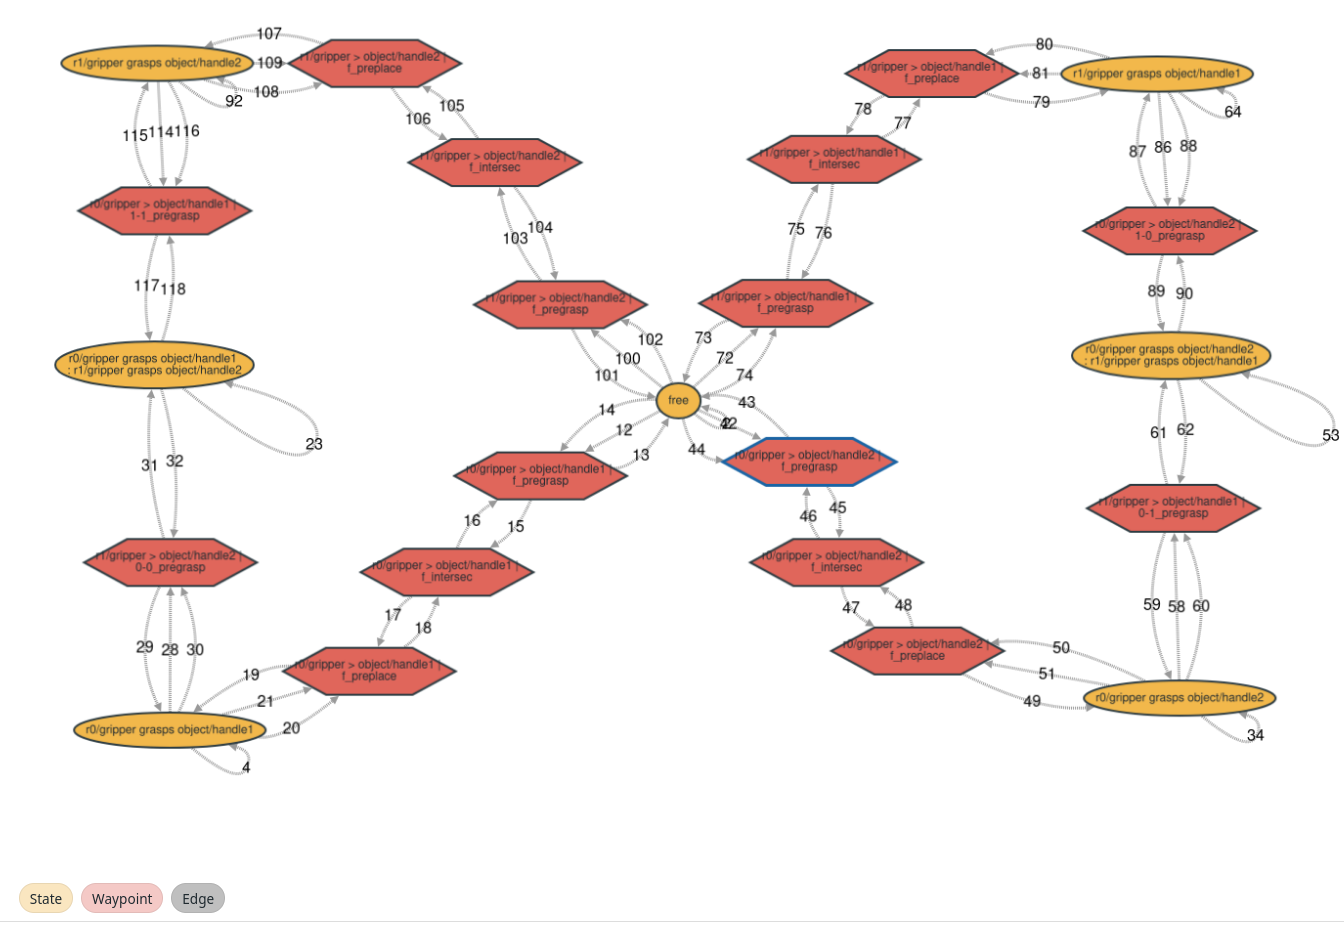
\includegraphics[width=.9\linewidth]{figures/constraint-graph-waypoints.png}
  \end{center}
\end{frame}

\begin{frame} {Motions on Lie groups}
  \parbox{.39\linewidth} {
    \begin{center}
      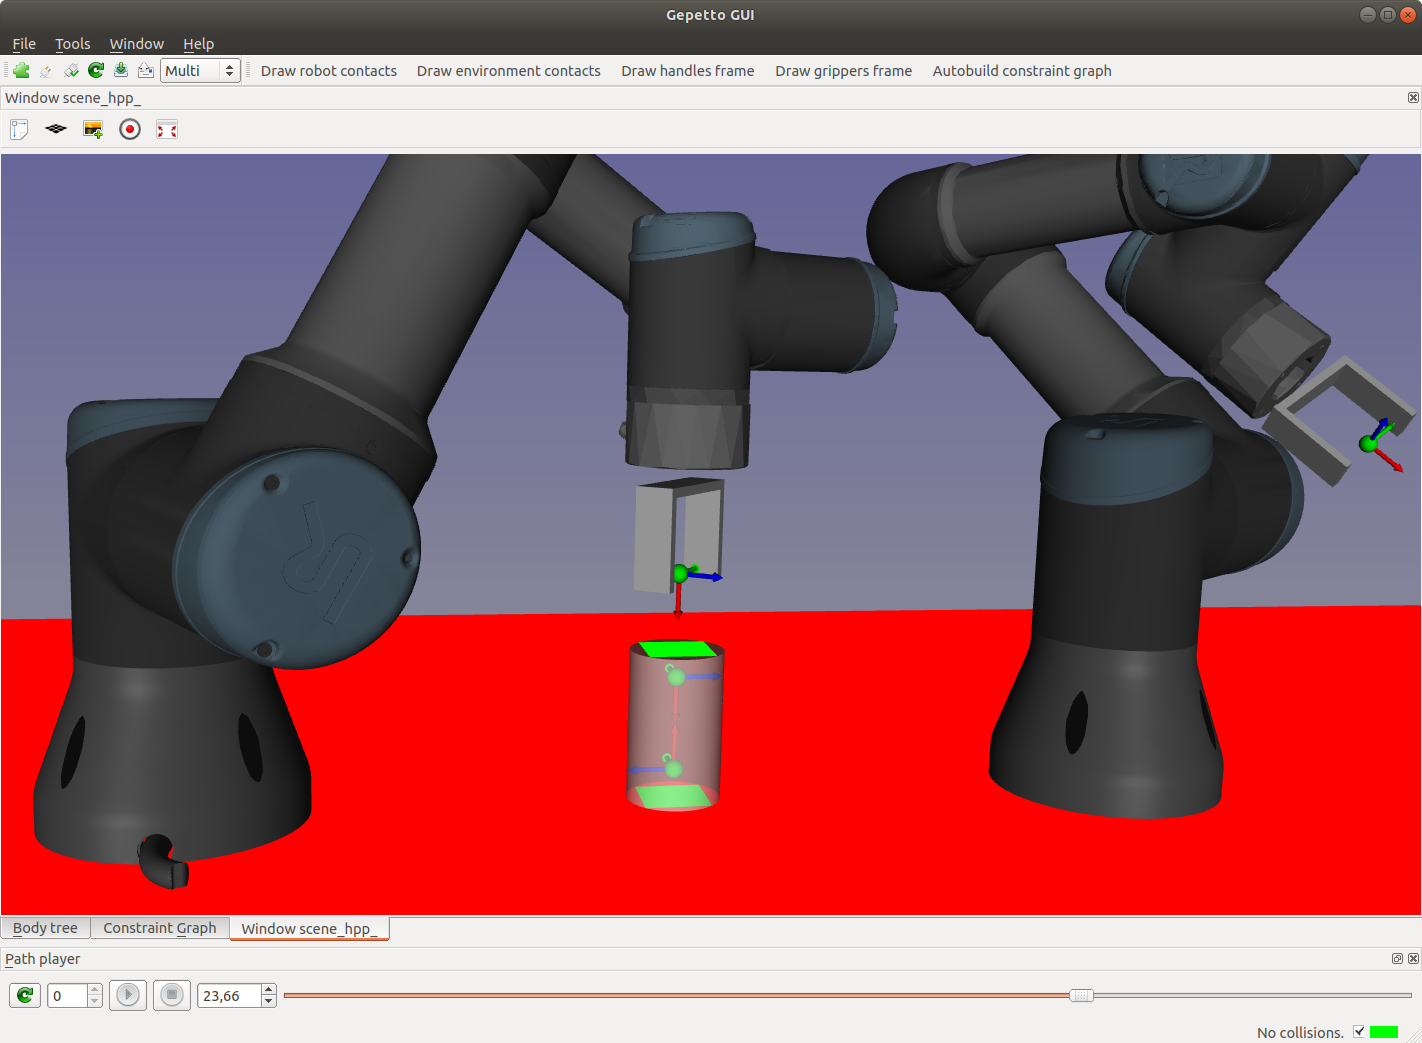
\includegraphics[width=\linewidth]{figures/manipulation-problem.png}
    \end{center}
  }
  \parbox{.57\linewidth} {
    The configuration space of a manipulation problem, here $\CS=\real^6\times\real^6\times SE(3)$
    \begin{itemize}
    \item is a Cartesian product of $\real^n$, $SO(2)$, $SO(3)$, $SE(2)$, $SE(3)$
    \end{itemize}
  }
  Each of those space share the properties of Lie groups.
\end{frame}

\begin{frame} {Motions on Lie groups}
  The elements and derivatives of those space are represented by vectors.
  \vskip .5cm
  \begin{center}
  \begin{tabular}{|l|c|c|}
    \hline
    Lie group type & configuration & velocity  \\
    \hline
    $\real^n$ & $\conf\in\real^n$ & $\mathbf{v}\in\real^n$ \\
    $SE(3)$ & $(x_1,x_2,x_3,p_1,\cdots,p_4)\in\real^7$ & $(\mathbf{v},\omega)\in\real^6$ \\
    $SE(2)$ & $(x_1,x_2,\cos\theta,\sin\theta)\in\real^4$ & $(\mathbf{v},\dot{\theta})\in\real^3$\\
    $SO(3)$ & $(p_1,p_2,p_3,p_4)\in\real^4$ & $\omega\in\real^3$\\
    $SO(2)$ & $(\cos\theta,\sin\theta)\in\real^2$ & $\dot{\theta}\in\real$\\
    \hline
  \end{tabular}
  \end{center}
  \parbox{.69\linewidth} {
  $$
  \left(q_1 \ \hdots \ q_6 \ q_7 \ \hdots \ q_{12} \ x \ y \ z \ p_1 \ p_2 \ p_3 \ p_4\right)
  $$
  }
  \parbox{.29\linewidth} {
    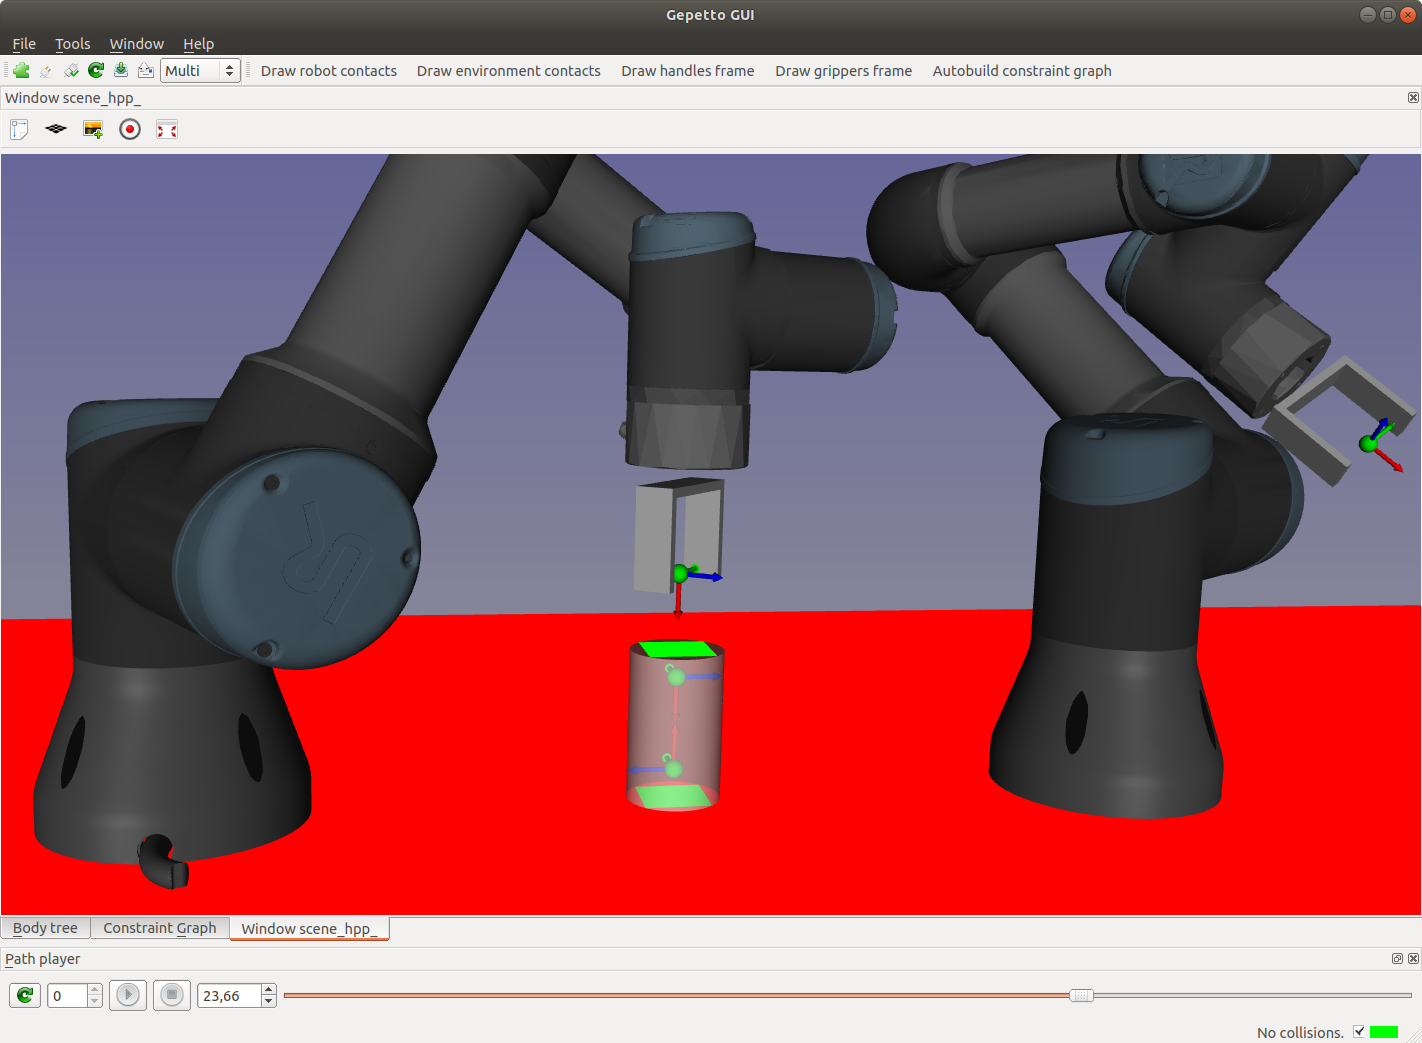
\includegraphics[width=\linewidth]{figures/manipulation-problem.png}
  }
\end{frame}

\begin{frame} {Motions on Lie groups}
  \begin{center}
  \begin{tabular}{|l|c|c|}
    \hline
    Lie group type & configuration & velocity  \\
    \hline
    $\real^n$ & $\conf\in\real^n$ & $\mathbf{v}\in\real^n$ \\
    $SE(3)$ & $(x_1,x_2,x_3,p_1,\cdots,p_4)\in\real^7$ & $(\mathbf{v},\omega)\in\real^6$ \\
    $SE(2)$ & $(x_1,x_2,\cos\theta,\sin\theta)\in\real^4$ & $(\mathbf{v},\dot{\theta})\in\real^3$\\
    $SO(3)$ & $(p_1,p_2,p_3,p_4)\in\real^4$ & $\omega\in\real^3$\\
    $SO(2)$ & $(\cos\theta,\sin\theta)\in\real^2$ & $\dot{\theta}\in\real$\\
    \hline
  \end{tabular}
  \end{center}
  $\conf$ Lie group element, $\mathbf{v}$ velocity
  \begin{itemize}
  \item $\exp \mathbf{v}$: element reached after moving with velocity $\mathbf{v}$ during unit time from origin.
  \item $\log \conf$ velocity that moves origin to $\conf$ in unit time.
  \end{itemize}
\end{frame}

\begin{frame} {Motions on Lie groups}
  $$\conf=
  \left(
  \begin{array}{ll}
    \real^6 &\left\{\begin{array}{l}q_1 \\ \vdots \\ q_6 \end{array}\right.\\
    \real^6 &\left\{\begin{array}{l} q_7 \\ \vdots \\ q_{12} \end{array}\right.\\
    SE(3)  &\left\{\begin{array}{l} x \\ y \\ z \\ p_1 \\ p_2 \\ p_3 \\ p_4\end{array}\right.
  \end{array}\right) \hspace*{1cm}
  \dconf=
  \left(
  \begin{array}{ll}
    \real^6 &\left\{\begin{array}{l}\dot{q}_1 \\ \vdots \\ \dot{q}_6 \end{array}\right.\\
    \real^6 &\left\{\begin{array}{l} \dot{q}_7 \\ \vdots \\ \dot{q}_{12} \end{array}\right.\\
    \real^6 &\left\{\begin{array}{l} \mathbf{v}\\ \omega \end{array}\right.
  \end{array}\right) \hspace*{1cm}
  $$
\end{frame}

\begin{frame} {Motions on Lie groups}
  $\exp$ and $\log$ are applied to each elementary Lie group.
  $$\conf=
  \left(
  \begin{array}{ll}
    \real^6 &\left\{\begin{array}{l}q_1 \\ \vdots \\ q_6 \end{array}\right.\\
    \real^6 &\left\{\begin{array}{l} q_7 \\ \vdots \\ q_{12} \end{array}\right.\\
    SE(3)  &\left\{\begin{array}{l} x \\ y \\ z \\ p_1 \\ p_2 \\ p_3 \\ p_4\end{array}\right.
  \end{array}\right) \hspace*{1cm}
  \log\conf=
  \left(
  \begin{array}{c}
    \begin{array}{l}q_1 \\ \vdots \\ q_6 \end{array}\\
    \begin{array}{l} q_7 \\ \vdots \\ q_{12} \end{array}\\
    \log\left(\begin{array}{l} x \\ y \\ z \\ p_1 \\ p_2 \\ p_3 \\ p_4\end{array}\right)
  \end{array}\right) \hspace*{1cm}
  $$
\end{frame}

\begin{frame} {Motions on Lie groups}
  $$\dconf=
  \left(
  \begin{array}{ll}
    \real^6 &\left\{\begin{array}{l}\dot{q}_1 \\ \vdots \\ \dot{q}_6 \end{array}\right.\\
    \real^6 &\left\{\begin{array}{l} \dot{q}_7 \\ \vdots \\ \dot{q}_{12} \end{array}\right.\\
    \real^6 &\left\{\begin{array}{l} \mathbf{v}\\ \omega \end{array}\right.
  \end{array}\right) \hspace*{1cm}
  \exp\dconf=
  \left(
  \begin{array}{c}
    \begin{array}{l}\dot{q}_1 \\ \vdots \\ \dot{q}_6 \end{array}\\
    \begin{array}{l} \dot{q}_7 \\ \vdots \\ \dot{q}_{12} \end{array}\\
    \exp\left(\begin{array}{l} \mathbf{v}\\ \omega \end{array}\right)
  \end{array}\right) \hspace*{1cm}
  $$
\end{frame}

\begin{frame} {Motions on Lie groups}
  \begin{itemize}
  \item $\conf\oplus\dconf\triangleq\conf.\exp\dconf\in\CS,\ \conf\in\CS, \dconf\in\TCS$,
    \begin{itemize}
    \item configuration reached from $\conf$ after following the constant velocity $\dconf$ during a unit time,
    \end{itemize}
  \item $\conf_2\ominus\conf_1\triangleq\log\left(\conf_1^{-1}.\conf_2\right)\in\TCS,\ \conf_1\in\CS, \conf_2\in\CS$,
    \begin{itemize}
    \item constant velocity that moves $\conf_1$ to $\conf_2$ in unit time.
      \end{itemize}
  \item $\conf_1 + t (\conf_2\ominus\conf_1)$
    \begin{itemize}
    \item linear interpolation between $\conf_1$ and $\conf_2$.
    \end{itemize}
  \end{itemize}
\end{frame}

\begin{frame} {Resources}
  \begin{itemize}
  \item \href{https://laas.hal.science/LAAS-GEPETTO/hal-02995125v2}{F.~Lamiraux and J.~Mirabel, Prehensile Manipulation Planning: Modeling, Algorithms and Implementation, IEEE transactions on Robotics, 2022},
  \item \href{https://humanoid-path-planner.github.io/hpp-doc}{Online documentation}
  \end{itemize}
\end{frame}
